% !TeX program = xelatex
\documentclass[11pt,a4paper]{article}
\usepackage{fontspec}
% File-based Windows font loading avoids MiKTeX's missing-font installer.
\IfFileExists{C:/Windows/Fonts/times.ttf}{%
\setmainfont{times.ttf}[Path=C:/Windows/Fonts/,BoldFont=timesbd.ttf,ItalicFont=timesi.ttf,BoldItalicFont=timesbi.ttf]
\setsansfont{arial.ttf}[Path=C:/Windows/Fonts/,BoldFont=arialbd.ttf,ItalicFont=ariali.ttf,BoldItalicFont=arialbi.ttf]
\setmonofont{consola.ttf}[Path=C:/Windows/Fonts/,BoldFont=consolab.ttf,ItalicFont=consolai.ttf,Scale=MatchLowercase]
}{%
\setmainfont{TeX Gyre Termes}
\setsansfont{TeX Gyre Heros}
\setmonofont{DejaVu Sans Mono}[Scale=MatchLowercase]
}
\usepackage[a4paper,left=25mm,right=23mm,top=24mm,bottom=24mm,headheight=15pt]{geometry}
\usepackage{graphicx,booktabs,tabularx,array,amsmath,float,needspace}
\usepackage[table]{xcolor}
\usepackage{fancyhdr,caption,titlesec,enumitem,tikz,url}
\usetikzlibrary{arrows.meta,positioning}
\definecolor{navy}{HTML}{17324D}
\definecolor{teal}{HTML}{217E87}
\definecolor{pale}{HTML}{EEF3F5}
\definecolor{ink}{HTML}{20262D}
\usepackage[unicode,colorlinks=true,linkcolor=navy,citecolor=teal,urlcolor=teal,bookmarksnumbered=true]{hyperref}
\hypersetup{pdftitle={DocuCheck AI - Báo cáo tiến độ tuần 1},pdfsubject={Submission I - Module 05},pdfauthor={Winner Winner Chicken Dinner: Nguyễn Văn Minh; Nguyễn Thành Trung}}
\renewcommand{\contentsname}{Mục lục}
\renewcommand{\refname}{Tài liệu tham khảo}
\renewcommand{\figurename}{Hình}
\renewcommand{\tablename}{Bảng}
\renewcommand{\thesection}{\Roman{section}}
\renewcommand{\thesubsection}{\arabic{section}.\arabic{subsection}}
\titleformat{\section}{\Large\sffamily\bfseries\color{navy}}{\thesection.}{.6em}{}
\titleformat{\subsection}{\large\bfseries\color{navy}}{\thesubsection}{.6em}{}
\titleformat{\subsubsection}{\normalsize\bfseries\color{navy}}{}{0pt}{}
\titlespacing*{\section}{0pt}{0pt}{14pt}
\titlespacing*{\subsection}{0pt}{13pt}{6pt}
\titlespacing*{\subsubsection}{0pt}{10pt}{4pt}
\setlength{\parindent}{0pt}
\setlength{\parskip}{6pt plus 1pt}
\linespread{1.08}
\setlength{\emergencystretch}{2em}
\raggedbottom
\setlength{\tabcolsep}{5pt}
\renewcommand{\arraystretch}{1.25}
\newcolumntype{P}[1]{>{\raggedright\arraybackslash}p{#1}}
\newcolumntype{Y}{>{\raggedright\arraybackslash}X}
\captionsetup{font=small,labelfont={bf,color=navy},justification=raggedright,singlelinecheck=false,skip=6pt}
\setlist{nosep,leftmargin=1.3em,topsep=4pt}
\pagestyle{fancy}
\fancyhf{}
\fancyhead[L]{\small\sffamily\color{navy}DOCUCHECK AI}
\fancyhead[R]{\small\sffamily\color{navy}BÁO CÁO TUẦN 1}
\fancyfoot[L]{\footnotesize\color{navy}Báo cáo tiến độ tuần 1 \enspace | \enspace 28.10.2026}
\fancyfoot[R]{\small\thepage}
\renewcommand{\headrulewidth}{.4pt}
\newcommand{\note}[1]{\par\begingroup\setlength{\fboxsep}{9pt}\noindent\colorbox{pale}{\parbox{\dimexpr\linewidth-18pt\relax}{#1}}\endgroup\par}
\urlstyle{tt}
\makeatletter
\g@addto@macro\UrlBreaks{\do\a\do\b\do\c\do\d\do\e\do\f\do\g\do\h\do\i\do\j\do\k\do\l\do\m\do\n\do\o\do\p\do\q\do\r\do\s\do\t\do\u\do\v\do\w\do\x\do\y\do\z\do\A\do\B\do\C\do\D\do\E\do\F\do\G\do\H\do\I\do\J\do\K\do\L\do\M\do\N\do\O\do\P\do\Q\do\R\do\S\do\T\do\U\do\V\do\W\do\X\do\Y\do\Z\do\0\do\1\do\2\do\3\do\4\do\5\do\6\do\7\do\8\do\9}
\makeatother
\begin{document}
\color{ink}

\begin{titlepage}
\thispagestyle{empty}
\centering
\setlength{\parskip}{0pt}
\vspace*{7mm}
{\sffamily\fontsize{16}{21}\selectfont\bfseries\color{navy}AI-VIETNAM}\par
\vspace{3mm}
{\sffamily\fontsize{11}{16}\selectfont KHÓA HỌC AIO2026}\par
\vspace{7mm}
{\color{navy!35}\rule{72mm}{.45pt}}\par
\vspace{25mm}
{\fontsize{23}{31}\selectfont\bfseries\color{navy}BÁO CÁO TIẾN ĐỘ TUẦN 1}\par
\vspace{5mm}
{\sffamily\fontsize{12}{17}\selectfont\color{teal}Submission I -- Module 05}\par
\vspace{17mm}
{\fontsize{29}{35}\selectfont\bfseries\color{navy}DocuCheck AI}\par
\vspace{3mm}
{\fontsize{14}{19}\selectfont Hệ thống xử lý và kiểm tra tài liệu}\par
\vspace{7mm}
{\fontsize{11}{16}\selectfont\itshape
Hiểu dữ liệu, xử lý tái lập và OCR baseline}\par
\vspace{24mm}
\begin{minipage}{114mm}
\normalsize
\renewcommand{\arraystretch}{1.65}
\begin{tabularx}{\linewidth}{@{}P{32mm}Y@{}}
\textbf{Tên nhóm} & Winner Winner Chicken Dinner\\
\textbf{Thành viên 1} & Nguyễn Văn Minh\\
\textbf{Thành viên 2} & Nguyễn Thành Trung\\
\end{tabularx}
\end{minipage}
\vfill
{\small Ngày lập báo cáo: 28 tháng 10 năm 2026}\par
\vspace{6mm}
{\footnotesize\href{https://github.com/AIVIETNAM-AIO-Heart208/DocuCheck-AI}{\textsf{github.com/AIVIETNAM-AIO-Heart208/DocuCheck-AI}}}\par
\vspace*{8mm}
\end{titlepage}

\section*{Tóm tắt}
DocuCheck AI hướng tới đọc thông tin trên ảnh biên lai tiếng Việt và cho phép người dùng kiểm tra lại kết quả trên ảnh gốc. Trong tuần đầu, nhóm tập trung vào ba việc: tìm hiểu dữ liệu, chuẩn bị quy trình xử lý có thể lặp lại và thiết lập một mốc OCR ban đầu.

Nhóm đã khảo sát 1.546 bản ghi biên lai, phân tích chất lượng ảnh và rà soát thủ công 40 ảnh được chọn để tìm rủi ro. Dữ liệu đã được chuẩn hóa, chia tập và kiểm tra để hạn chế ảnh trùng giữa các tập. Trên 231 ảnh đánh giá nội bộ, Tesseract đã tạo kết quả nhận dạng cho toàn bộ ảnh. Kết quả này giúp nhóm thấy rõ những khó khăn của cả dữ liệu lẫn cách đánh giá OCR; chưa phải mức chất lượng có thể dùng để trích xuất thông tin tự động.

\section{Mục tiêu và phạm vi tuần 1}
Ảnh biên lai thường có ánh sáng không đều, chữ nhỏ, giấy nhăn hoặc nền phức tạp. Dự án đặt mục tiêu xác định bốn thông tin chính: tên nơi bán, địa chỉ, thời điểm giao dịch và tổng tiền. Mỗi thông tin cần gắn với vị trí trên ảnh để người dùng có thể kiểm tra lại. Trong tuần 1, nhóm xây dựng nền dữ liệu và OCR ban đầu cho mục tiêu đó \cite{mcocr,repo}.

Đây là báo cáo tiến độ nghiên cứu. Nhóm chưa huấn luyện mô hình trích xuất bốn trường thông tin, chưa đánh giá độ chính xác theo từng trường và chưa hoàn thành ứng dụng cho người dùng.

\section{Kết quả 1: Hiểu dữ liệu biên lai}
\subsection{Quy mô và đặc điểm dữ liệu}
Bản dữ liệu đang sử dụng gồm 1.155 ảnh biên lai train và 391 ảnh validation chính thức. Phần train có 6.585 vùng gán nhãn cho các trường thông tin cần tìm. Ngoài ra còn có transcript toàn trang và một bộ 6.585 ảnh cắt nhỏ dành riêng cho nhận dạng chữ. Nhóm giữ các nguồn này tách biệt vì ảnh cắt nhỏ chưa được xác nhận là các vùng thông tin trên cùng biên lai.

\begin{table}[H]
\caption{Quy mô dữ liệu nhóm đã khảo sát.}\label{tab:inventory}
\begin{tabularx}{\linewidth}{@{}Yr@{}}
\toprule
\textbf{Thành phần} & \textbf{Số lượng} \\\midrule
Bản ghi biên lai & 1.546 \\
Ảnh train có nhãn thông tin & 1.155 \\
Ảnh validation chính thức & 391 \\
Vùng thông tin được gán nhãn trên ảnh train & 6.585 \\
Vùng transcript toàn trang & 40.868 \\
Ảnh cắt nhỏ cho tác vụ nhận dạng chữ riêng & 6.585 \\
\bottomrule
\end{tabularx}
\end{table}

Các nhãn tập trung vào tên nơi bán, địa chỉ, thời điểm giao dịch và tổng tiền. Số vùng gán nhãn không đồng nghĩa số ảnh: một ảnh có thể có nhiều vùng cho cùng một trường. Trong 1.155 ảnh train, có 947 ảnh được gán đủ bốn loại trường; việc thiếu nhãn chưa chứng minh trường đó không xuất hiện trên ảnh.

Phần lớn ảnh train có bố cục dọc; độ sáng và độ rõ của chữ thay đổi đáng kể (Hình~\ref{fig:eda}). Những khác biệt này giúp nhóm chọn ảnh cần kiểm tra kỹ hơn.

\begin{figure}[H]
\centering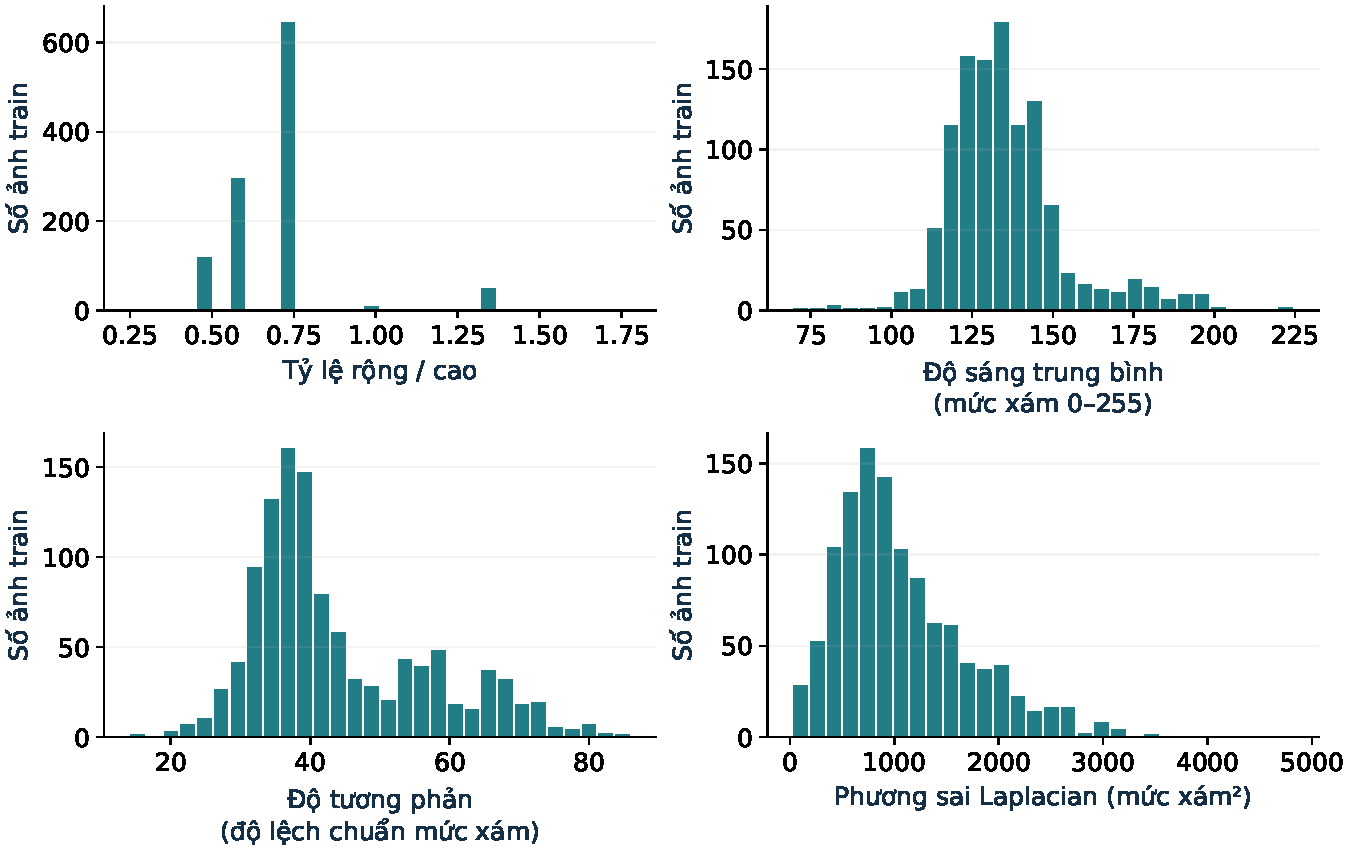
\includegraphics[width=\linewidth]{figures/eda_distributions.pdf}
\caption{Phân bố hình dạng, độ sáng, tương phản và mức biến thiên chi tiết của 1.155 ảnh train.}\label{fig:eda}
\end{figure}

\subsection{Rà soát nhãn và ảnh trùng}
Nhóm rà soát 40 ảnh được chọn có chủ đích để dễ phát hiện vấn đề. Kết quả ghi nhận 6 ảnh đúng, 32 ảnh có ít nhất một vấn đề và 2 ảnh chưa thể kết luận. Những vấn đề thường gặp gồm thiếu vùng cần gán nhãn, nhãn sai hoặc vị trí vùng không khớp nội dung trên ảnh.

\begin{table}[H]
\caption{Một số vấn đề ghi nhận khi rà soát 40 ảnh.}\label{tab:audit}
\begin{tabularx}{\linewidth}{@{}YrY@{}}
\toprule
\textbf{Vấn đề} & \textbf{Số ảnh} & \textbf{Ví dụ về tác động} \\\midrule
Thiếu nhãn cho thông tin nhìn thấy & 21 & Mô hình có thể học từ dữ liệu chưa đầy đủ \\
Gán sai loại thông tin & 8 & Tên nơi bán có thể bị hiểu thành trường khác \\
Vùng đánh dấu sai vị trí & 6 & Chữ trong vùng không khớp giá trị cần lấy \\
Chữ khó đọc & 3 & Cần kiểm tra thủ công hoặc xử lý ảnh tốt hơn \\
\bottomrule
\end{tabularx}
\end{table}

\noindent\textit{Các nhóm vấn đề có thể trùng trên cùng một ảnh. Mẫu 40 ảnh được ưu tiên để tìm lỗi, nên tỷ lệ 32/40 không đại diện cho toàn bộ dữ liệu.}

Kiểm tra trên toàn tập còn ghi nhận 115 biên lai có vùng chú thích sai hình học. Nhóm đã nhận diện và giữ thông tin về các trường hợp này để tránh coi chúng là nhãn chuẩn trong những bước sau.

Nhóm phát hiện 20 bản ghi train trùng chính xác với ảnh trong tập validation chính thức và đã cách ly chúng khỏi tập huấn luyện, đánh giá nội bộ. Có thêm 36 cặp ảnh gần giống cần xem lại bằng mắt để xác định có cùng giao dịch hay không. Kết quả hiện tại giúp giảm nguy cơ đánh giá lạc quan do ảnh trùng; chưa thể khẳng định đã tìm hết mọi trường hợp gần trùng.

\section{Kết quả 2: Chuẩn bị dữ liệu cho các bước tiếp theo}
Nhóm đã xây dựng quy trình đọc ảnh và nhãn, chuẩn hóa về cùng một cấu trúc, ghi lại các vấn đề của dữ liệu gốc và chia tập theo nhóm ảnh trùng chính xác. Dữ liệu gốc được giữ nguyên để có thể đối chiếu khi cần. Quy trình kiểm tra cả bản ghi lẫn ảnh tương ứng; tổng cộng 8.131 bản ghi ảnh, gồm 1.546 biên lai và 6.585 ảnh cắt nhỏ, đã qua kiểm tra cấu trúc.

\begin{figure}[H]
\centering
\begin{tikzpicture}[node distance=5mm and 6mm, every node/.style={font=\small,align=center}, box/.style={draw=teal,rounded corners=2pt,fill=pale,text width=39mm,minimum height=12mm}, arr/.style={-{Latex[length=2mm]},thick,color=teal}]
\node[box] (raw) {Ảnh và nhãn gốc};
\node[box,right=of raw] (norm) {Chuẩn hóa và\\ghi nhận vấn đề};
\node[box,right=of norm] (split) {Cách ly ảnh trùng\\và chia tập};
\node[box,below=of split] (check) {Kiểm tra dữ liệu\\đầu ra};
\draw[arr] (raw)--(norm);\draw[arr] (norm)--(split);\draw[arr] (split)--(check);
\end{tikzpicture}
\caption{Quy trình chuẩn bị dữ liệu đã hoàn thành trong tuần 1.}\label{fig:pipeline}
\end{figure}

\begin{table}[H]
\caption{Kết quả chia 1.546 bản ghi biên lai.}\label{tab:splits}
\begin{tabularx}{\linewidth}{@{}YrY@{}}
\toprule
\textbf{Nhóm} & \textbf{Số ảnh} & \textbf{Vai trò} \\\midrule
Train nội bộ & 904 & Dữ liệu cho bước phát triển mô hình \\
Dev nội bộ & 231 & Dữ liệu đánh giá OCR ban đầu \\
Cách ly do trùng validation & 20 & Không dùng để huấn luyện hoặc đánh giá nội bộ \\
Validation chính thức & 391 & Tập ảnh được giữ riêng \\\midrule
Tổng cộng & 1.546 & \\
\bottomrule
\end{tabularx}
\end{table}

Quy trình có cách giữ lại bản ghi kèm cảnh báo, bỏ bản ghi lỗi hoặc dừng khi gặp lỗi. Việc lặp lại hai lần chuẩn bị dữ liệu trong hồ sơ kiểm tra cho cùng kết quả đầu ra; bộ kiểm thử của dự án ghi nhận 106 trường hợp đạt. Đây là bằng chứng về tính nhất quán của quy trình. Chất lượng nhãn vẫn cần được rà soát riêng: một bản ghi hợp lệ về cấu trúc vẫn có thể được gán sai nội dung.

\section{Kết quả 3: OCR ban đầu và bài học rút ra}
Nhóm sử dụng Tesseract với mô hình tiếng Việt để nhận dạng chữ và vị trí trên ảnh \cite{tesseract}. Trên toàn bộ 231 ảnh dev nội bộ, chương trình tạo kết quả cho 231 ảnh, với 26.859 vùng từ được nhận dạng. Đây là mốc đầu tiên để quan sát lỗi và cải thiện cách xử lý biên lai, chưa phải kết quả trích xuất bốn trường thông tin.

\begin{table}[H]
\caption{Kết quả OCR trên 231 ảnh dev nội bộ.}\label{tab:ocrresults}
\begin{tabularx}{\linewidth}{@{}YrY@{}}
\toprule
\textbf{Chỉ số} & \textbf{Kết quả} & \textbf{Cách hiểu} \\\midrule
Ảnh có kết quả nhận dạng & 231/231 & Chương trình xử lý hết tập ảnh dev \\
Vùng từ được nhận dạng & 26.859 & Đầu ra để xem chữ và vị trí trên ảnh \\
CER trên toàn tập (tỷ số) & 1,8725 & Sai khác ký tự với transcript tham chiếu \\
WER trên toàn tập (tỷ số) & 2,1448 & Sai khác token với transcript tham chiếu \\
\bottomrule
\end{tabularx}
\end{table}

CER và WER ở đây so chữ nhận dạng với transcript sau khi ghép các vùng trên ảnh. Cả hai tỷ số có thể lớn hơn 1 khi số ký tự hoặc token chèn thêm nhiều hơn độ dài tham chiếu. Giá trị cao hiện tại phản ánh đồng thời lỗi nhận dạng, nhãn tham chiếu chưa sạch và cách ghép vùng chữ; không thể dùng riêng chúng để kết luận Tesseract đọc sai bao nhiêu phần trăm chữ trên ảnh.

\begin{figure}[H]
\centering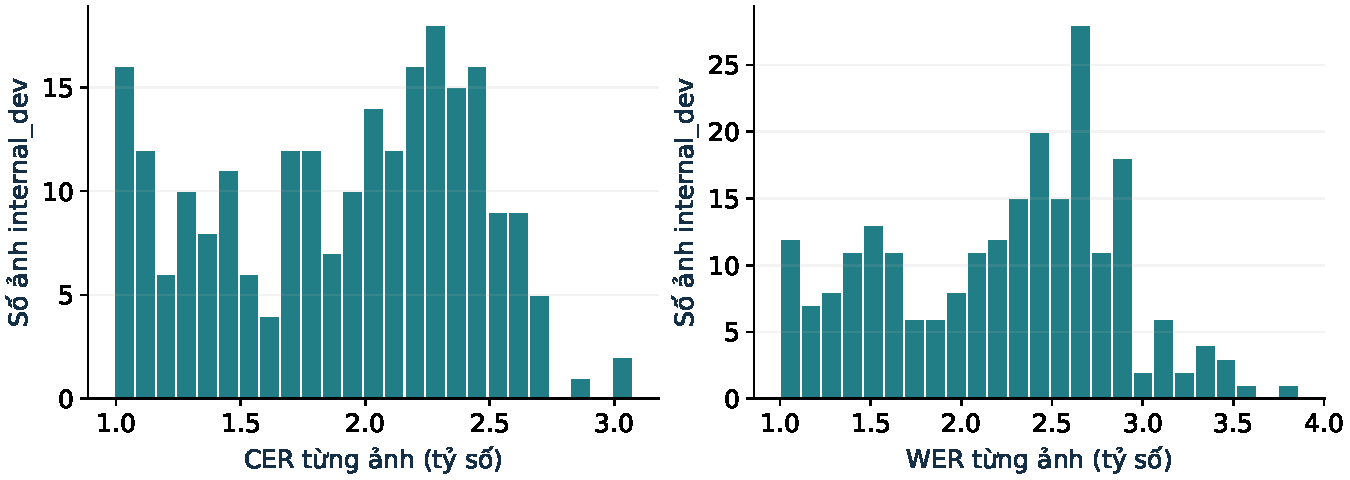
\includegraphics[width=\linewidth]{figures/ocr_error_distribution.pdf}
\caption{Mức sai khác OCR giữa các ảnh dev không đồng đều; biểu đồ dùng cùng cách ghép vùng với chỉ số trong Bảng~\ref{tab:ocrresults}.}\label{fig:ocrerror}
\end{figure}

Phân tích kết quả cho thấy có 1.886 vùng chữ tham chiếu không nhận được vùng từ tương ứng, trong khi 10.488 vùng từ dự đoán nằm ngoài các vùng tham chiếu hợp lệ. Điều này cho thấy việc đối chiếu chữ dự đoán với nhãn hiện có còn khó khăn. Trước khi so sánh các mô hình OCR, nhóm cần kiểm tra lại nhãn và thống nhất cách đánh giá.

\section{Kết luận và hướng tiếp theo}
Ba mục tiêu tuần 1 đã có kết quả cụ thể: nhóm hiểu quy mô và rủi ro của dữ liệu, có quy trình chuẩn bị dữ liệu có thể lặp lại, và có một mốc OCR chạy trên tập dev. Kết quả quan trọng nhất là đã xác định được những điểm có thể làm sai lệch việc huấn luyện hoặc đánh giá sau này: nhãn thiếu/sai, ảnh gần trùng và cách ghép vùng khi tính lỗi OCR.

Bước tiếp theo là rà soát các nhãn cần dùng cho trích xuất thông tin, xác định các cặp ảnh gần trùng, cải thiện cách đánh giá OCR và xây dựng mô hình nhận diện bốn trường trên biên lai. Các kết quả này sẽ cần được đo ở mức thông tin trích xuất và kiểm tra trực tiếp trên ảnh trước khi hướng tới ứng dụng cho người dùng.

\begin{thebibliography}{9}
\bibitem{mcocr} MC-OCR Challenge. \textit{Mobile captured receipts OCR}. \url{https://www.rivf2021-mc-ocr.vietnlp.com/}
\bibitem{tesseract} Tesseract OCR. \textit{Tài liệu sử dụng}. \url{https://tesseract-ocr.github.io/tessdoc/}
\bibitem{repo} DocuCheck AI. \textit{Kho mã dự án}. \url{https://github.com/AIVIETNAM-AIO-Heart208/DocuCheck-AI}
\end{thebibliography}
\end{document}
